\subsection*{CAUTION: Danger ahead!}\index{genomic prediction!caveats}

This all seems very promising, but a word of caution is in
order. Several papers, including one by Peter Turchin, have suggested
that there is strong evidence for selection on polygenic scores
associated with height using the same data set of 253,288 individuals
I referred to earlier~(references in Berg et
al.~\cite{Berg-etal-2018}). Specifically, these studies suggested (a)
that there is a cline in polygenic scores from south-to-north in
Europe (taller phenotypes predicted in the north) and (b) that the
cline is too steep to be accounted for by neutrual evolution. Berg et
al.~\cite{Berg-etal-2018} re-examined these claims using new data
available from the UK
Biobank~(\url{https://www.bdi.ox.ac.uk/research/uk-biobank}), which
includes a host of information on individual phenotypes as well as
genome-wide genotypes for the 500,000 individuals included in the
sample.\footnote{Although all of the samples are from the UK, one of
  the data sets Berg et al.~\cite{Berg-etal-2018} studied included
  individuals of European, but non-UK, ancestry.} They failed to
detect evidence of a cline in polygenic scores in their
analysis~(Figure~\ref{fig:UK-biobank}).

\begin{figure}
  \begin{center}
    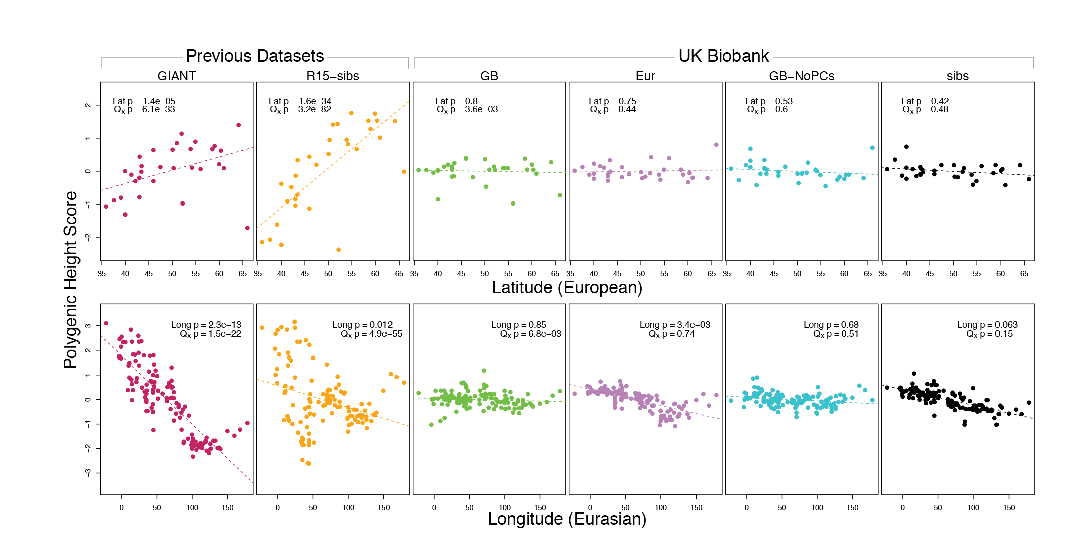
\includegraphics[width=\textwidth]{UK-biobank.eps}
  \end{center}
  \caption{Polygenic score as a function of latitude and longitude for
    several different GWAS data sets.}\label{fig:UK-biobank}
\end{figure}

In thinking about this result, it's important to understand that Berg
et al.~\cite{Berg-etal-2018} did something a bit different from what
we did, but it's exactly what you'd want to do if polygenic scores
worked. They estiamted polygenic scores from each of the data sets
identified in the figure. Then they used those scores to estimate
polygenic scores for a new set of samples derived from the 1000
Genomes and Human Origins projects.\footnote{See Berg et
  al.~\cite{Berg-etal-2018} for details.} Think about it. A polygenic
score doesn't do us a whole lot of good if all it lets us do is to
predict (with uncertainty) a phenotype we already know. The hope is
that we can use the polygenic score to predict phenotypes for
individuals when we know their genotype but not their phenotype. What
this result shows is that extrapolation of a regression beyond the
range of variation included in the sample from which it was estimated
can be very problematic.

